\documentclass[a4paper,twocolumn]{article}
\usepackage[utf8]{inputenc}
\usepackage{graphicx}
\usepackage{epstopdf}
\usepackage{amsmath}
\usepackage{amssymb}
\setlength{\columnsep}{0.8cm}
\def\code#1{\texttt{#1}}
\begin{document}

%%%%%%% title
\title{Polymer chains}
\date{9 April 2016}
\author{Ludwig Rasmijn\\ 4106644 \and Sebastiaan Lokhorst\\ 4005058 \and Shang-Jen Wang\\ 4215974}
\maketitle
%%%%%%%

\begin{abstract}
	The behavior of polymer chains in 2D is investigated by simulating a random walk using two different methods.
	Both the Rosenbluth and the Pruning-Enriched Rosenbluth Method (PERM) are used, with six choices for successive beads, which have a probability based on the energy of the new bead, which is modeled with the Lennard-Jones potential.
	The end-to-end distance $R$ as a function of the length of the polymer, expressed in the number of beads $N$, is studied for both methods. It is concluded that they are related by $R \propto (N-1)^{0.75}$, which is in accordance with literature such as Thijssen\cite{thijssen}.
\end{abstract}

\section{Introduction}
From an early stage polymer physics has been used to develop Monte Carlo algorithms. These algorithms depend on the problem of interest: is the polymer in a melt or in a solution. In this report the focus is on a dilute polymer solution.\\ \\ 
The polymer model is a self-avoiding walk in 2 dimensions, where each effective monomer is a fixed distance from the nearest neighbour. The interaction between the beads is modeled by the Lennard-Jones potential:

\begin{equation}\label{eq:lennardjones}
	V_{LJ}=4\epsilon \left[ \left( \frac{\sigma}{r} \right)^{12} - \left( \frac{\sigma}{r} \right)^{6} \right]\text{.}
\end{equation}

Where $\epsilon = 0.25$ (natural units), and $\sigma = 0.8$, given that the distance between monomers is equal to $1$.
\section{Methods}
\subsection{Rosenbluth algorithm}
The Rosenbluth algorithm is a Monte-Carlo method to generate polymers, which will avoid high-energy conformations when adding new beads to the polymer.\cite{rosenbluth} This method uses six evenly spaced ($2\pi /6$) discrete angles with a random offset for which the new bead can be added to the polymer, as shown in fig. \ref{fig:roulette}. It will avoid any improbable conformations by adding the next bead with a probability proportional to $\exp(-E(\theta)/(k_BT))$, where $E(\theta)$ is the interaction energy of the new bead with the rest of the polymer, and $\theta$ is the angle between the new bead and the previous two beads. The weight for each angle $\theta_j$ is calculated with:
\begin{equation}\label{eq:weight}
	w_j^{(l)}=\exp(-E(\theta_j)/(k_BT)) \text{,}
\end{equation}\label{eq:sumweight}
where $j$ is the number of the angle and $l$ is the bead that is being added. The sum of all the weights can be expressed as:
\begin{equation}
	W^{(l)}=\sum_j \exp(-E(\theta_j)/(k_BT)) \text{.}
\end{equation}
So angle $j$ is accepted with a probability $w_j^{(l)}/W^{(l)}$.\\
The weight of the total polymer is given by:
\begin{equation}\label{eq:polweight}
	\text{PolWeight}=\prod_l W^l\text{.}
\end{equation}

\begin{figure}
	\centering
	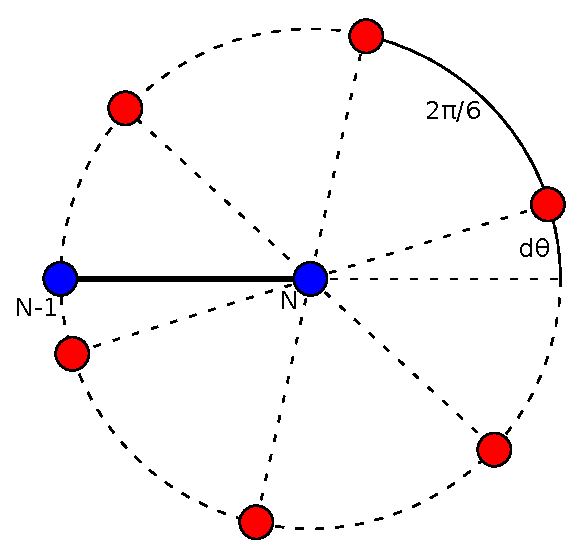
\includegraphics[width=0.5\linewidth]{roulette.eps}
	\caption{Choosing bead $N+1$ out of  one of the six possible angles $\theta_j$}
	\label{fig:roulette}
\end{figure}

\subsection{Pruned-enriched Rosenbluth method}
A method which suppresses the high energy configuration better than the Rosenbluth method is the pruned-enriched Rosenbluth method (PERM) by Grassberger \cite{grassberger}. This method removes configurations with a high energy and low weight and multiplies configurations with a low energy and high weight. This way, the high-weight and thus more important configurations, are studied more closely.

Two thresholds $\code{UpLim}$ and $\code{LowLim}$ are used to define `low' and `high' weights. If at any polymer length the $\code{PolWeight} > \code{UpLim}$, then two members of this polymer are created when adding the next bead and each are given a $\code{PolWeight}$ which half the PolWeight of the original polymer. This is called `enriching'. If at any polymer length the $\code{PolWeight} < \code{LowLim}$, then the polymer will be removed with a probability of $1/2$. If the polymer is not removed, then the $\code{PolWeight}$ is multiplied by $2$. This will make sure that the distribution does not change. This is called `pruning'.

The choice of $\code{UpLim}$ and $\code{LowLim}$ depends on the average weight $\code{AvWeight}$ at polymer length $L$.
The average weight is updated for every polymer that reaches that length. $\code{UpLim}$ and $\code{LowLim}$ are expressed as a ratio of the average weight and the weight $\code{Weight3}$ corresponding to the shortest length (3 beads):
\begin{equation}\label{eq:uplim}
    \code{UpLim}=\alpha \cdot \code{AvWeight}/\code{Weight3} \text{,}
\end{equation}
\begin{equation}\label{eq:lowlim}
    \code{LowLim}=\alpha \cdot \code{AvWeight}/\code{Weight3} \text{.}
\end{equation}
A good value for $\alpha$ for $\code{UpLim}$ is 2 and for $\code{LowLim}$ 1.2. It is possible that $\alpha$ is dependent on $L$, but this dependency can be removed by multiplying the weight of the polymer by a constant at each step. This constant should be near $1/(0.75N_{\theta})$, where $N_{\theta}$ is the number of possible angles. 

\section{Results and Discussion}
The polymer simulation was used to study the end-to-end distance of a polymer $R$, illustrated in fig. \ref{fig:end-to-end-distance}.

\begin{figure}
	\centering
	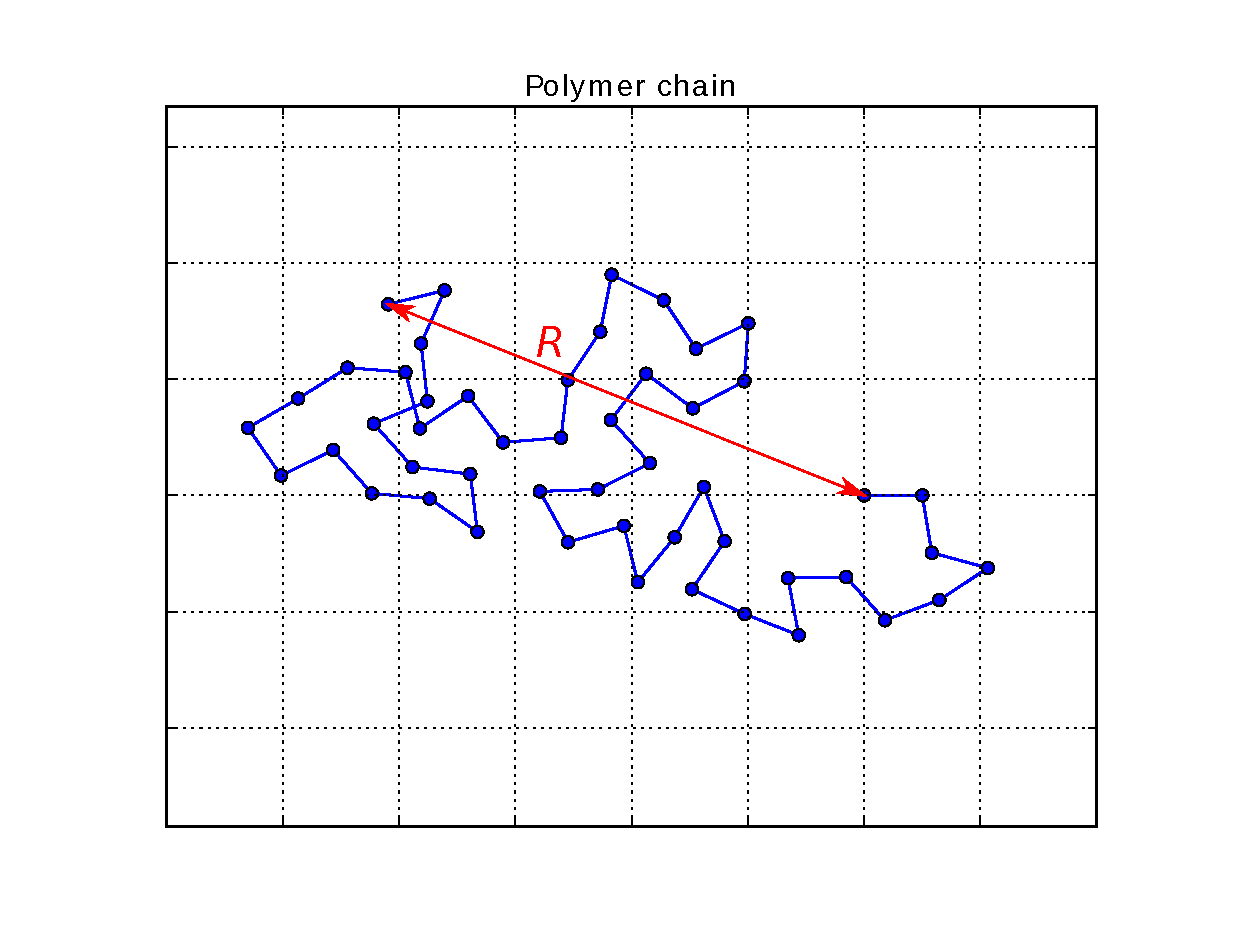
\includegraphics[width=\linewidth]{end-to-end-distance.eps}
	\caption{End-to-end distance $R$ for a polymer of length $N=50$}
	\label{fig:end-to-end-distance}
\end{figure}

An average value for $R^2$ can be obtained by simulating multiple polymers and then averaging them with the weight of the polymers.

The end-to-end distance $R$ of the polymer should scale with:
\begin{equation}\label{eq:end-to-end}
	R \propto {N_s}^\nu \text{,}
\end{equation}
where $N_s$ is the number of segments, and $\nu = 0.75$ in two dimensions.\cite{thijssen}

This means that the results should fit:
\begin{equation}\label{eq:end-to-end-sq}
	R^2 = a(N-1)^{1.5} \text{,}
\end{equation}
Where $a$ is a scaling constant.

The square end-to-end distance $R^2$, determined with the regular Rosenbluth algorithm is shown in fig. \ref{fig:r2_noperm}. Note that the population stays constant but the error for large $N$ is quite large, even for such an high population.

\begin{figure}
	\centering
	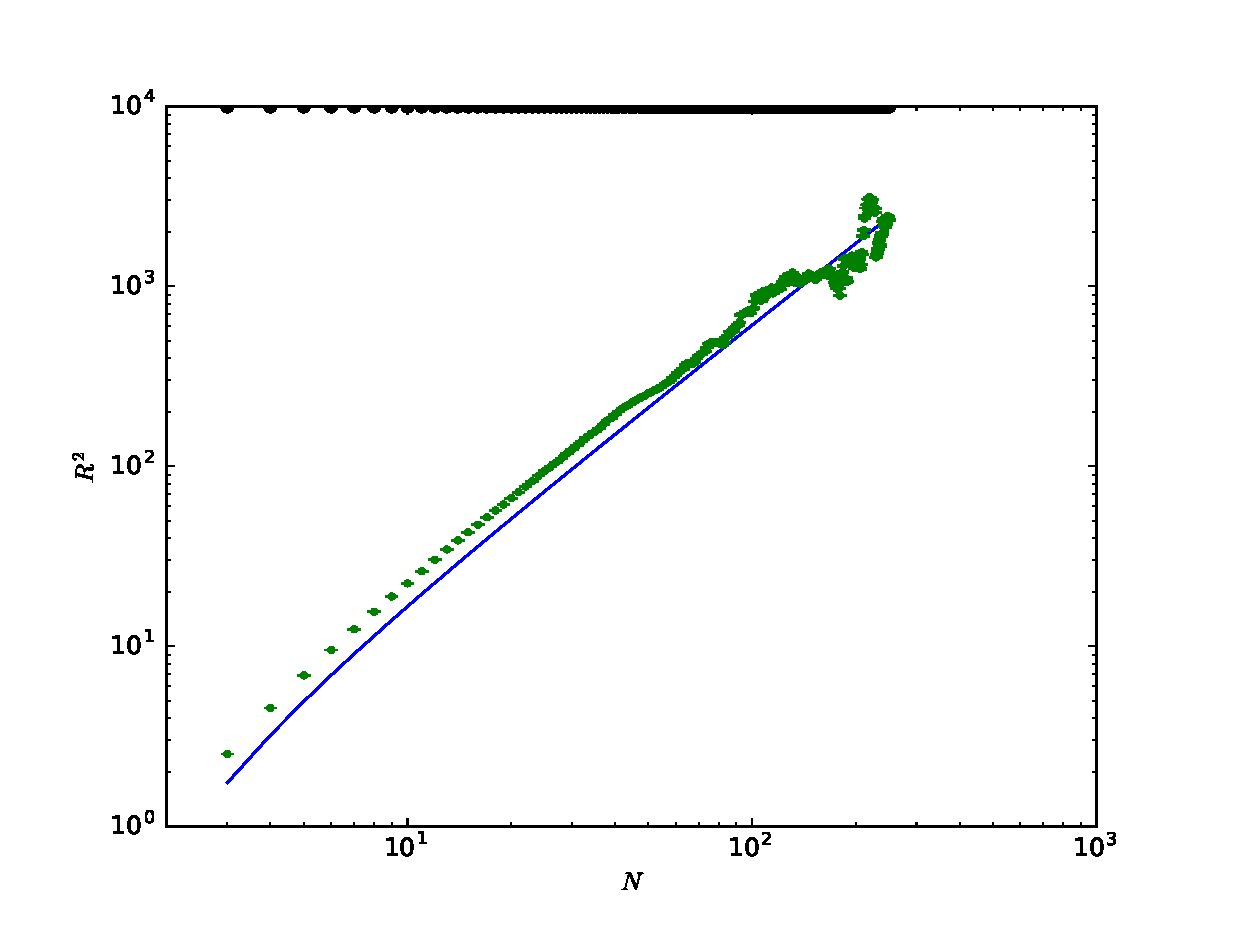
\includegraphics[width=\linewidth]{r2_noperm_10000run.eps}
	\caption{The average $R^2$ as a function of the number of beads $N$. Fitted to the function $R^2 = 0.62(N-1)^{1.5}$. The black dots represent the population size, which is constant at 10,000}
	\label{fig:r2_noperm}
\end{figure}

The same $R^2$, but now determined with the PERM algorithm, is shown in fig. \ref{fig:r2_perm}. Note that while the population is \emph{smaller} than for the regular Rosenbluth method, the error for large $N$ is much smaller. This is because low-weight (and thus irrelevant) configuration are suppressed, and the computation focuses on the high-weight (relevant) population.

Because in the PERM case the computation is focused on the relevant polymers, it is much more efficient. The computation time scales with $\sum_{N} \code{population}(N)$. When comparing the population of the regular Rosenbluth and the PERM algorithm, they both are relatively constant. However the error in the case of the PERM algorithm is much better, even with a population which is ten times as small.

\begin{figure}
	\centering
	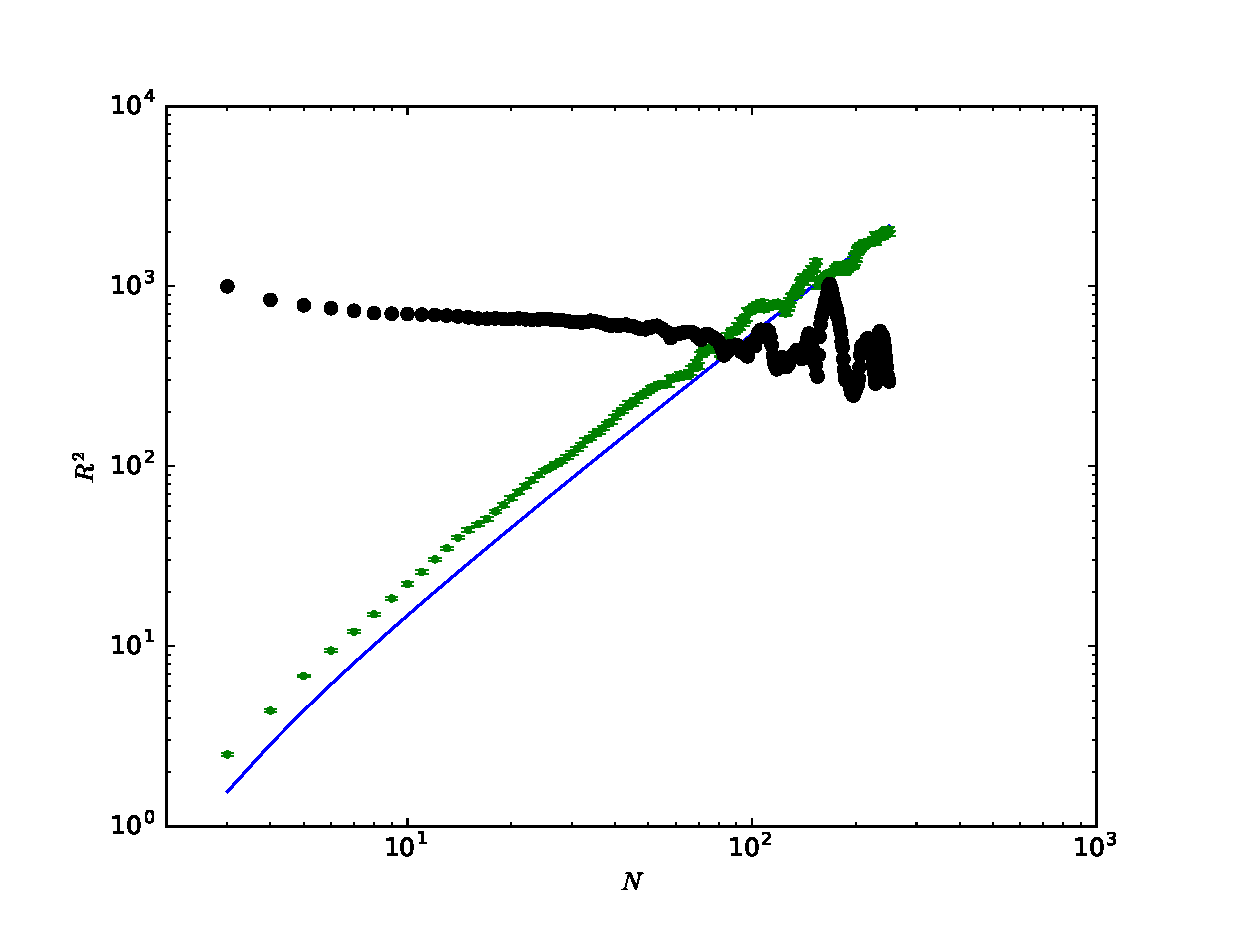
\includegraphics[width=\linewidth]{r2_perm_1000run.eps}
	\caption{The average $R^2$ as a function of the number of beads $N$, computed with PERM. The black dots represent the population size, which fluctuates around 1,000}
	\label{fig:r2_perm}
\end{figure}

\section{Conclusion}

In this study, polymer chains were simulated using the Rosenbluth and Pruning-Enriched Rosenbluth Method (PERM). Polymers were grown to a length of up to 250 beads. The end-to-end distance was investigated and found to be in accordance with literature, namely obeying the relationship $R^2 = a(N-1)^{1.5}$ with $a \approx 0.6$. It was found that the PERM method is superior in finding high-probability configurations and thus requiring a smaller population to achieve a more precise result.

\begin{thebibliography}{9}
\bibitem{thijssen}
	J.M. Thijssen (2007)\\
	$\textit{Computational Physics}$.\\
	Cambridge University Press
\bibitem{rosenbluth}
	M. N. Rosenbluth and A. W. Rosenbluth (1955)\\
	$\textit{Monte Carlo Calculation of the} $ \\ $\textit{Average Extension of Molecular Chains}$\\
	J. Chem. Phys. 23, 356
\bibitem{grassberger}
	P. Grassberger (1997)\\
	$\textit{Pruned-enriched Rosenbluth method:} $ \\ $\textit{Simulation of $\theta$ polymers of chain length}$ \\ $\textit{up to 1 000 000}$.\\
	Phys. Rev. E, 56, 3682–93
\end{thebibliography}

\end{document}
